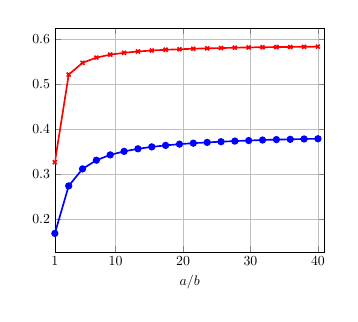
\begin{tikzpicture}[scale=0.5]
\begin{axis}[xlabel=$a/b$,ymajorgrids=true,xmajorgrids=true,xmin=1,xmax=41,xtick={1,10,20,30,40}]
%%%%%%%%%%% NATURAL CONFIGURATION
\addplot[Blue,mark=*,very thick] coordinates {(1.0,0.168781687817) (3.05263157895,0.274434323291) (5.10526315789,0.312241017147) (7.15789473684,0.331556999781) (9.21052631579,0.343371854771) (11.2631578947,0.351188775046) (13.3157894737,0.356866726562) (15.3684210526,0.361161506352) (17.4210526316,0.364452065573) (19.4736842105,0.367277356984) (21.5263157895,0.3693952729) (23.5789473684,0.371136342942) (25.6315789474,0.372686884764) (27.6842105263,0.374017424385) (29.7368421053,0.375282700195) (31.7894736842,0.376391132332) (33.8421052632,0.377343247117) (35.8947368421,0.377975358701) (37.9473684211,0.378718524027) (40.0,0.379203792038) };
%%%%%%%%%%% MODIFIED CONFIGURATION
\addplot[Red,mark=x,very thick] coordinates {(1.0,0.327083270833) (3.05263157895,0.521791533705) (5.10526315789,0.548055480555) (7.15789473684,0.559609806624) (9.21052631579,0.566176714399) (11.2631578947,0.570259386804) (13.3157894737,0.573250469347) (15.3684210526,0.575399438205) (17.4210526316,0.576991033068) (19.4736842105,0.578179466005) (21.5263157895,0.579278950684) (23.5789473684,0.580283697574) (25.6315789474,0.580817387121) (27.6842105263,0.581651079669) (29.7368421053,0.582253190953) (31.7894736842,0.5827068797) (33.8421052632,0.583105304737) (35.8947368421,0.583295306637) (37.9473684211,0.583636362679) (40.0,0.584005840058) };
\end{axis}
\end{tikzpicture}
%%% Local Variables:
%%% mode: latex
%%% TeX-master: "../../mainManuscript"
%%% End:
